\subsection {Overview}

\subsubsection{Relay Control}
\begin{figure}
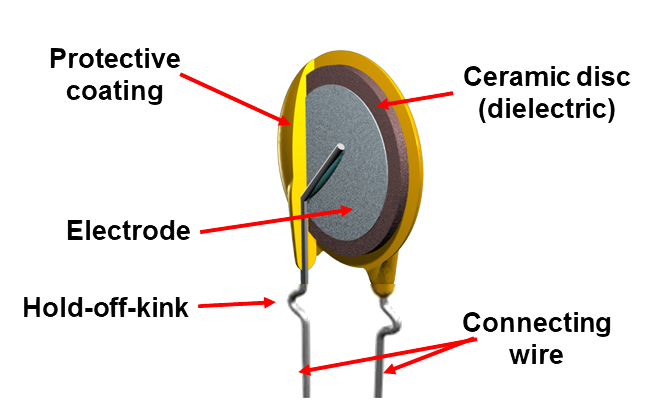
\includegraphics[keepaspectratio=true,scale=.5]{./figures/testImage.png}
\centering
%    \cite{capSite_df_vs_temp}
\caption{Relay Control Circuitry}
\label{cdlRelayCir_fig}
\end{figure}


Each relay is controlled with independent circuitry as shown in Figure: \ref{cdlRelayCir_fig}. The basic operation is that the input control signal (active high) switches either 5V or GND to the low side of the relay's coil. A ringback diode in series with a small valued resistor is in place to limit the coil's inductive spike while switching. Additionally there is a resistor + LED to indicate when an individual relay is active.

\subsection {Protection}

This subsection will explain the protection circuitry used to isolate parts of the circuit from the high DC voltage in the event of a failure.

\subsection {AC Signal Injection}

This subsection will cover the circuitry and supporting tech needed to inject an AC signal onto the DUT.

\subsection {AC voltage Measurement}

This subsection describes the AC voltage amplitude and phase measurements. 

\subsection {Rise and Fall Times}

This subsection describes the circuitry used to mesaure the rise and fall times of the DUT.


